\section{Anwendungen}
\label{chapApp}
Für das Betriebssystem wurde eine Reihe von Anwendungen entwickelt, welche teilweise in das Betriebssystem kompiliert wurden, teilweise aber auch für das Starten von einem externen Speichermedium vorgesehen sind. Einige der implementierten Anwendung steuern einen \textit{Moving Head} über das \ac{DMX}-Protokoll. Im Folgenden werden die Anwendungen und teilweise Implementierungsdetails erläutert.

\subsection{Implementierte Anwendungen}
Die folgende Tabelle \ref{table:apps} zeigt eine Auflistung der implementierten Anwendungen, welche in den Kernel kompiliert wurden und jeweils eine kurze Beschreibung.

\begin{table}[H]
\begin{tabular}{p{4cm} | p{10cm}}
  \textbf{Name} & \textbf{Beschreibung}
  \\ \hline
  \textit{hello} & Eine \textit{HelloWorld}-Applikation. Die Anwendung nimmt ebenfalls einen Parameter entgegen, welcher die Ausgabe beeinflußt
  \\
  \textit{cwd} & Ausgabe der aktuellen \ac{CWD}.
  \\
  \textit{more} & Ausgabe einer Textdatei.\newline
  Verwendung: \texttt{more <filename>}
  \\
  \textit{cd} & Wechseln der aktuellen \ac{CWD}.\newline
  Verwendung: \texttt{cd [.. | <directory>]}
  \\
  \textit{ps} & Ausgabe der aktuell laufenden Prozesse
  \\
  \textit{kill} & Forciertes Beenden eines Prozesses. \newline Verwendung: \texttt{kill <pid>}
  \\
  \textit{ping} & Demonstrationsanwendung für die Interprozesskommunikation (Empfänger). \newline Verwendung: \texttt{ping \&} (Für das Starten im Hintergrund)
  \\
  \textit{pong} & Demonstrationsanwendung für die Interprozesskommunikation (Sender). \newline Verwendung: \texttt{pong <message>}
  \\
  \textit{uptime} & Gibt die aktuelle Laufzeit des Betriebssystems in Millisekunden aus.
  \\
  \textit{dmx} & Demonstrationsanwendung für die Ansteuerung eines \textit{Moving Heads}.
  \\
  
 \end{tabular}
 \caption{Übersicht der implementierten Anwendungen}
 \label{table:apps}
\end{table}

Tabelle \ref{table:extapps} zeigt eine Auflistung der Anwendungen, welche von einem externen Speichermedium gestartet werden können, sowie eine kurze Beschreibung.
Für Anwendungen welche von einem externen Speichermedium gestartet werden gilt grundsätzlich, dass diese mit vollem Anwendungsnamen und Dateiendung, beispielsweise also \texttt{app.bin}, gestartet werden müssen. Liegen Anwendungen im Verzeichnis \texttt{/bin} können diese ohne Dateiendung gestartet werden, beispielsweise also \texttt{app}.

\begin{table}[H]
\begin{tabular}{p{4cm} | p{10cm}}
  \textit{empty.bin} & Eine Anwendung ohne jegliche Ausgabe.\newline Verwendung: \texttt{empty.bin}
  \\
  \textit{nptest.bin} & Demonstriert die Abhandlung des Nulladressenproblems.\newline Verwendung: \texttt{nptest.bin}
  \\
  \textit{hellow~1.bin} & Eine erweiterte "Hallo, Welt"-Anwendung.\newline Verwendung: \texttt{hellow~1.bin [<name>]}
    \\
  \textit{dmxtest.bin} & Eine Demonstration der Ansteuerung von \textit{Moving Heads}.\newline Verwendung: \texttt{dmxtest.bin}
    \\
  \textit{echo} & Kommando zum Ausgeben eines beliebigen Texts. \newline Verwendung: \texttt{echo <param1> [<param2>, ...]}
    \\
  \textit{dd} & Ein \textit{High-Level}-Treiber für die Ansteuerung von \textit{Moving Heads}, welcher mehrere \textit{Namespaces} für die Interprozesskommunikation öffnet und Befehle abarbeitet. \newline Verwendung: \texttt{dd \&} (Zum Starten als Hintergrundprozess)
  \\
  \textit{ipcd} & Eine Hilfsanwendung für die Auflistung und das Ansprechen von Prozessen mittels Interprozesskommunikation. \newline Verwendung:\newline \texttt{ipcd -l} (Zum Ausgeben aller offenen \textit{Namespaces})
  \newline \texttt{ipcd -s <channel> <string>} (Sendet den gegebenen Parameter an den \textit{Namespace})
  \newline \texttt{ipcd -c <channel> <num> [<num>, ...]} (Sendet die gegebenen Parameter als Rohdaten zum gegebenen \textit{Namespace})
  \\
 \end{tabular}
 \caption{Übersicht der implementierten externen Anwendungen}
 \label{table:extapps}
\end{table}


\subsection{Implementierte \ac{DMX}-Anwendung}
Im Allgemeinen gibt es mehrere verschiedene Spezifikationen für das \ac{DMX}-Protokoll. Im folgenden wird eine dieser unterschiedlichen Spezifikation erläutert und anschließend zu Vergleichszwecken verwendet. Abbildung \ref{fig:DMX-512-Protocol} dient zur Veranschaulichung des \ac{DMX}-512 Protokolls. Die hier ersichtliche Spezifikation wurde als Treiber für die \ac{DMX}-Anwendung implementiert.

% http://mc.mikrocontroller.com/de/dmx512.php
% TODO: add reference to this webside

\begin{figure}[H]
	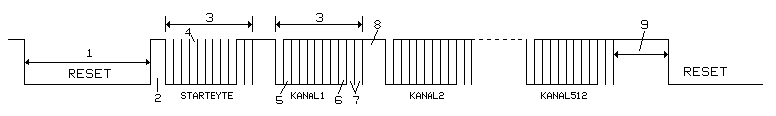
\includegraphics[scale=0.60]{chapters/userapplication/figures/dmxproto}
	\caption{DMX Protokoll \cite{dmx}}
	\label{fig:DMX-512-Protocol}
\end{figure}

Tabelle \ref{table:DMX-512-Protocol} beschreibt die einzeln nummerierten Markierungen aus Abbildung \ref{fig:DMX-512-Protocol}.

\begin{table}[H]
\begin{tabular}{p{1.5cm} | p{6.5cm} | p{1cm} | p{1cm} | p{1cm} | p{1cm}}
  \textbf{Nummer} & \textbf{Signalname} & \textbf{Min.} & \textbf{Typ.} & \textbf{Max.} & \textbf{Einheit} \\ 
  \hline
  1 & Reset & 88.0 & 88.0 & - & $\mu$s \\
  2 & Mark zwischen Reset- und Startbyte & 8.0 & - & 1 s & $\mu$s \\
  3 & Frame-Zeit & 43.12 & 44.0 & 44.48 & $\mu$s \\
  4 & Startbit & 3.92 & 4.0 & 4.08 & $\mu$s \\
  5 & LSB (niederwertigstes Datenbit) & 3.92 & 4.0 & 4.08 & $\mu$s \\
  6 & MSB (höchstwertigstes Datenbit) & 3.92 & 4.0 & 4.08 & $\mu$s \\
  7 & Stopbit & 3.92 & 4.0 & 4.08 & $\mu$s \\
  8 & Mark zwischen Frames (Interdigit) & 0 & 0 & 1.0 & s \\
  9 & Mark zwischen Paketen & 0 & 0 & 1.0 & s \\
  - & Reset-Reset (Paketabstand) & 1094 & - & - & $\mu$s \\
 \end{tabular}
 \caption{Eigenschaften des DMX-512-Protokolls}
 \label{table:DMX-512-Protocol}
\end{table}

Die Übertragungsgeschwindigkeit ist bei allen Protokollarten identisch und beträgt $250kBaud$, d.h. jedes Bit hat eine Dauer von $4\mu s$. Das \ac{DMX}-Protokoll besitzt $512$ verschiedene Kanäle, wobei jeder Kanal mithilfe eines Datenbytes gesteuert wird. In Abbildung \ref{fig:DMX-512-Protocol} ist ersichtlich, dass jedes übertragene Datenbyte zusätzlich ein Startbit sowie zwei Stopbits besitzt. Somit ergeben sich für jeden Kanal genau elf Bits.\\

Die Implementierung des oben erläuterten Protokolls stellt sich teilweise als herausfordernd dar. In Abbildung \ref{fig:DMX-Edge} und Abbildung \ref{fig:DMX-Offset-Byte} sind jeweils zwei Messergebnisse ersichtlich, welche von den \ac{DMX}-Geräten nicht korrekt interpretiert werden konnten.\\
\begin{figure}[H]
	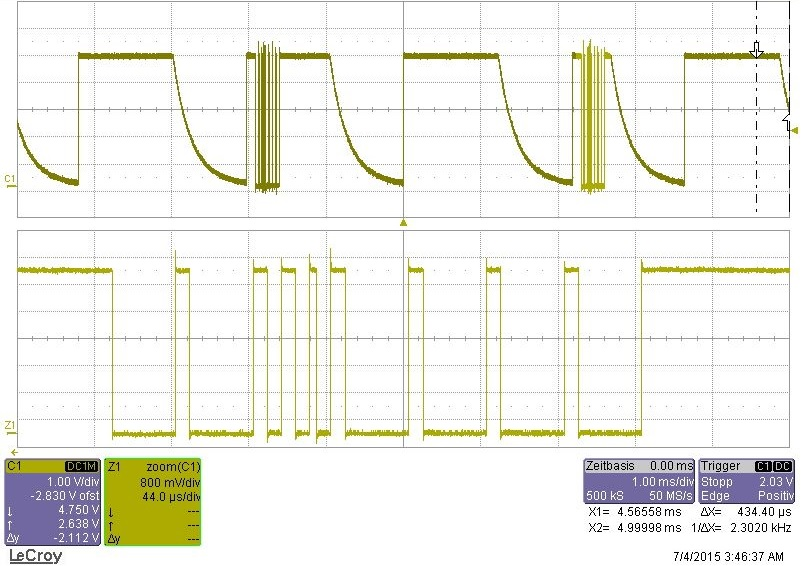
\includegraphics[scale=0.6]{chapters/userapplication/figures/DMX-Edge}
	\caption{DMX Protokoll: Problem fallende Flanke}
	\label{fig:DMX-Edge}
\end{figure}

\begin{figure}[H]
	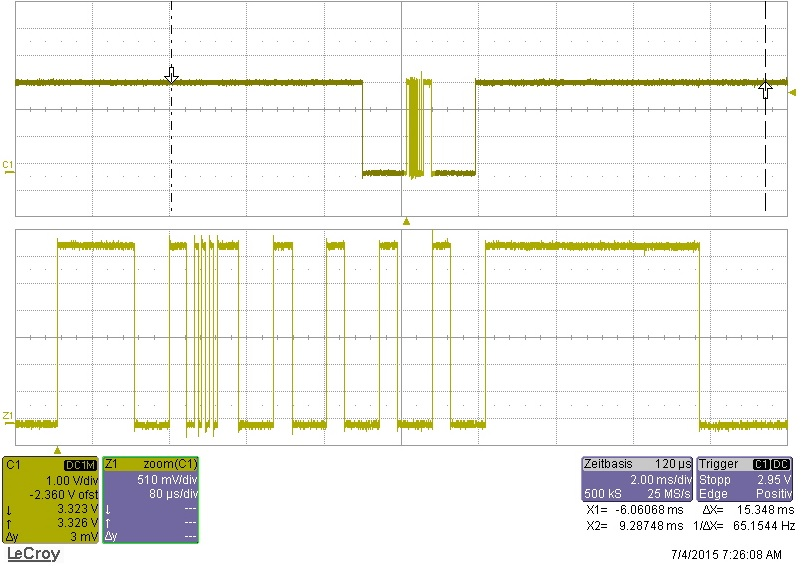
\includegraphics[scale=0.6]{chapters/userapplication/figures/DMX-Offset-Byte}
	\caption{DMX Protokoll: Problem Offset Byte}
	\label{fig:DMX-Offset-Byte}
\end{figure}

Abbildung \ref{fig:DMX} zeigt schließlich das Messergebnis des erfolgreich und funktionierenden \ac{DMX}-Protokolls.
\begin{figure}[H]
	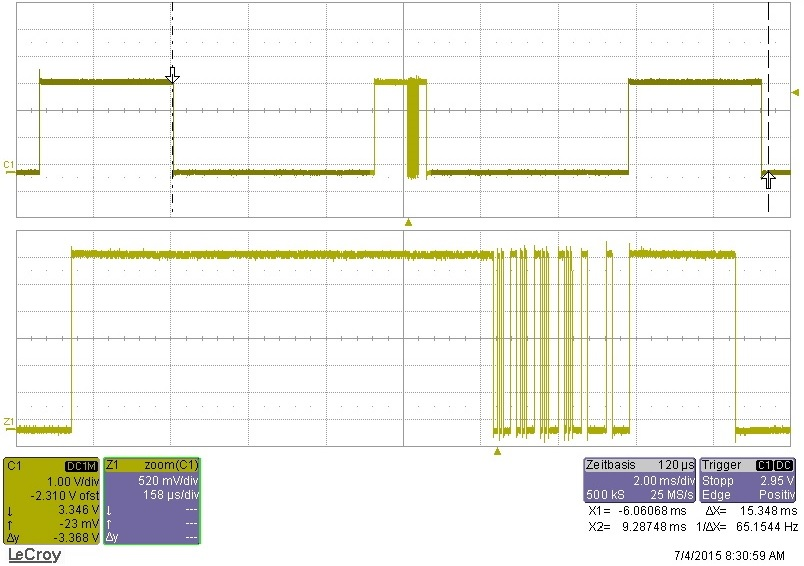
\includegraphics[scale=0.6]{chapters/userapplication/figures/DMX}
	\caption{Funktionierendes DMX Protokoll}
	\label{fig:DMX}
\end{figure}

\pagebreak 